%% --- setup, packages, and commands -------------------------------------------
\documentclass[10pt, a4paper]{article}
\usepackage{geometry}

% Libertine Font
\usepackage{libertine, libertinust1math}
\usepackage[T1]{fontenc}
\usepackage[utf8]{inputenc}
\usepackage{bm}

\usepackage[nocomma]{optidef}

% creates \uline command with standardized underline height to mathstrut level
\newcommand{\uline}[1]{\underline{\vphantom{\mathstrut}#1}}

% figures
\usepackage{graphicx}
\usepackage{caption}
\usepackage{subcaption}
\usepackage{float}

% columnshttps://www.overleaf.com/project/6343697362ae47178db077e2
\usepackage{multicol}

% graphs
\usepackage{tikz}

% code snippets with command \code
\usepackage{xcolor}
\definecolor{lightgray}{gray}{0.95}
\definecolor{gray}{rgb}{0.25,0.25,0.25}
\definecolor{green}{rgb}{0,0.6,0}
\definecolor{purple}{rgb}{0.58,0,0.82}
\definecolor{blue}{rgb}{0.58,0,0.82}
\newcommand*{\code}[1]{\colorbox{lightgray}{\texttt{\footnotesize{#1}}}}
\usepackage{listings}
\lstdefinestyle{mystyle}{
    backgroundcolor=\color{lightgray},
    commentstyle=\color{green},
    keywordstyle=\color{magenta},
    numberstyle=\tiny\color{gray},
    stringstyle=\color{purple},
    basicstyle=\ttfamily\scriptsize,
    identifierstyle=\color{black},
    breakatwhitespace=false,
    breaklines=true,
    captionpos=b,
    keepspaces=true,
    numbers=left,
    numbersep=5pt,
    showspaces=false,
    showstringspaces=false,
    showtabs=false,
    tabsize=4,
}
\lstset{style=mystyle}

% Section formatting
\usepackage{color,soul}
\usepackage{titlesec}
\titlespacing\section{0em}{1em}{0.5em}
\titleformat{\section}{\normalfont\huge\bfseries}{}{0em}{}

\titlespacing\subsection{0em}{1.6em}{0.2em}
\titleformat{\subsection}{\normalfont\LARGE}{}{0em}{}

\titleformat{\subsubsection}{\normalfont\Large}{}{0em}{}
\titleformat{\paragraph}[runin]{\normalfont\normalsize}{}{0em}{\indent$\bullet$\enspace}
\titleformat{\subparagraph}[runin]{\normalfont\normalsize\bfseries}{}{0em}{}

% Prompt uses code style with a $ terminal prompt and a newline at the end
\newcommand*{\prompt}[1]{\code{\$ #1}}

% Add tilde, ~ character with command \home
\newcommand{\home}{\char`\~}

% Hyperlinks with commands \link and \reference for external and item links
\usepackage[breaklinks]{hyperref}
\hypersetup{pdfborder={0 0 0}} % remove border around links
\newcommand*{\link}[2]{\href{#1}{\uline{#2}}} % underlined \link
\newcommand*{\reference}[2]{\hyperref[#1]{\uline{#2}}} % underlined \reference
\newcommand*{\largebf}[1]{\begin{large}\textbf{#1}\end{large}}
\newcommand*{\largeit}[1]{\begin{large}\textit{#1}\end{large}}

% Title Setup
\title{\begin{Huge}\textsc{CS 839 Project Proposal}\end{Huge}}
\author{Connor Bailey, Cole Dilanni, and Spencer Schoenberg}
\date{\today}

\geometry{
    top=1in,
    inner=1in,
    outer=1in,
    bottom=1in,
    headheight=3em,
    headsep=1em,
    footskip=.5in
}

\begin{document}

\maketitle

\section{Overview}
Models can have difficulties handling color. For example, a model trained on only red cars might not be able to extrapolate the features it's learned to blue cars. To the best of our knowledge, while models such as CNNs are translation invariant there don’t exist any true color-invariant models. This stems from the problem of how to define color invariance. For our project, we hope to modify existing model architectures to promote color invariance. We define color invariance as having the same or very similar output when the input image’s color is dramatically changed without changing the image's semantic meaning. For example, a dramatic change could be changing the order of the RGB channels as this would greatly modify the color of the image while keeping the semantic meaning intact.

\begin{figure}[H]
    \centering
    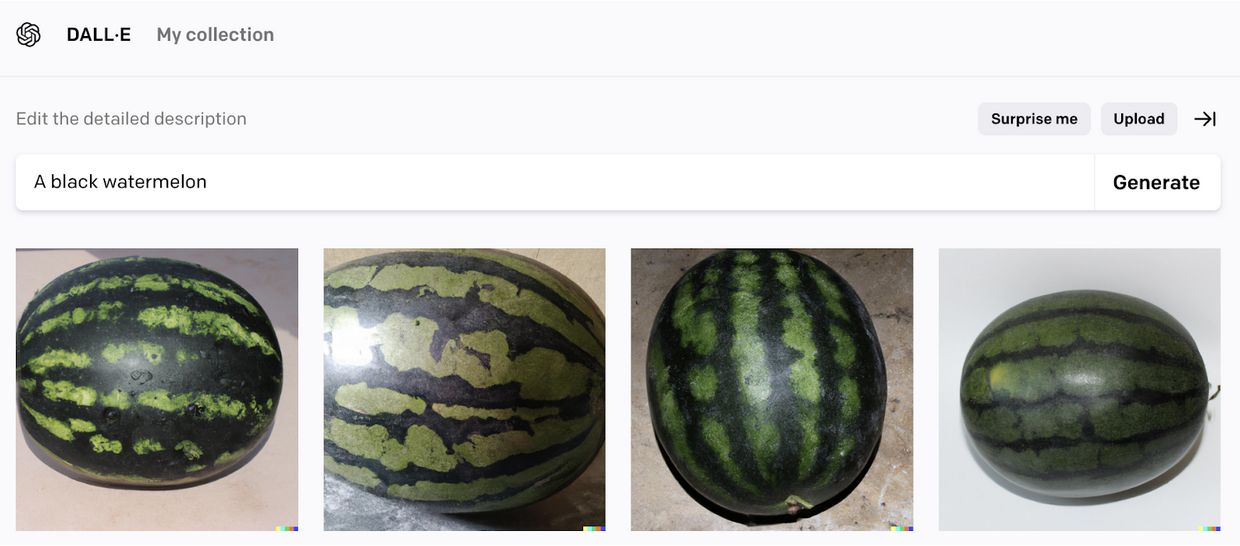
\includegraphics[width=0.75\textwidth]{1.png}
    \caption{One example of how current models fail with color changes is DALL-E 2, a state-of-the-art image generator. When given the prompt of “A black watermelon”, even this model cannot disentangle the object and its color.}
    \label{model3}
\end{figure}

Our goal is to investigate the input type (RGB versus different, more suitable color spaces) and the initial neural network layer(s) to better handle color shifts. In doing so, we aim to create a “color invariant” CNN/transformer model. We will investigate this classification model’s performance on standard datasets such as MNIST and CIFAR-10 to ensure removing the true input color values does not drastically harm the model’s performance. Given a functional “color invariant” model, we expect it to focus more on object shape rather than textures (as current CNNs are biased to do).

Using the top-performing color space and color distance metric for creating a color invariant model, we will then transfer the model’s framework to build a color invariant discriminator within a GAN. If the discriminator does not have specific image color information, we hope the generator will learn to make out of distribution colored images that still have the semantic meaning/shape as the training dataset. For example, we could train on black/white MNIST images and generate red/green images. Not only this, but since the color invariance is local, we hope to generate images such as a blue horse with a red mane and a green tail. This color-OOD generating GAN can then be used as a data augmentation technique for supervised learning tasks to force new models to be less biased toward object color/texture.

\section{Related Work}

There has already been work to compare color spaces as input to regular convolutional neural networks \cite{Sachin18}. These works will guide us in choosing the color spaces to test, but do not address changing the model structure to view colors as relative to each other.

Other works have investigated illumination invariance \cite{Ng08}\cite{Choi10} \cite{Gevers99} and various data augmentations to simulate color invariance  \cite{Xu22}\cite{Zhang16}, but illumination invariance does not effectively handle color changes in the object and it is impossible to search over the entire span of possible data augmentations while training a color invariant model. These prior works would also likely fail under conditions where the colors of individual parts of an object are changed. Consider the example of a blue horse with a red main and a green tail. Classical data augmentation techniques would not be able to simulate this color shift because they generally look at the image as a whole. Yet, a human would still be able to recognize such a horse because the semantic meaning hasn't changed.

\section{Technical Approach}
\noindent We plan to employ CNNs and color space embeddings (RGB, HSV, XYZ, LAB) to develop our color invariant model. We will modify the existing convolutional layer to use a self-attention mechanism that takes relative distances (euclidean and learned) between each pixel in the kernel instead of the base RGB values. This modified, color invariant layer will replace the first convolutional layer in a ResNet-50 model, leaving the rest of the model the same. Only the first layer of the classification/discriminator model needs to be converted for color invariance because only it deals with the color space directly.

\section{Experiments}
\begin{itemize}
    \item Build, test, and compare both regular and color invariant models
          \begin{itemize}
              \item Test performance on MNIST
              \item Test performance on CIFAR-10
              \item Test with augmented versions of above datasets
              \item Compare models’ loss/accuracy
          \end{itemize}
    \item Investigate different color spaces/color distance metrics
          \begin{itemize}
              \item RGB
              \item CIELAB/spherical color spaces with meaningful distance metrics

                    \begin{figure}[H]
                        \centering
                        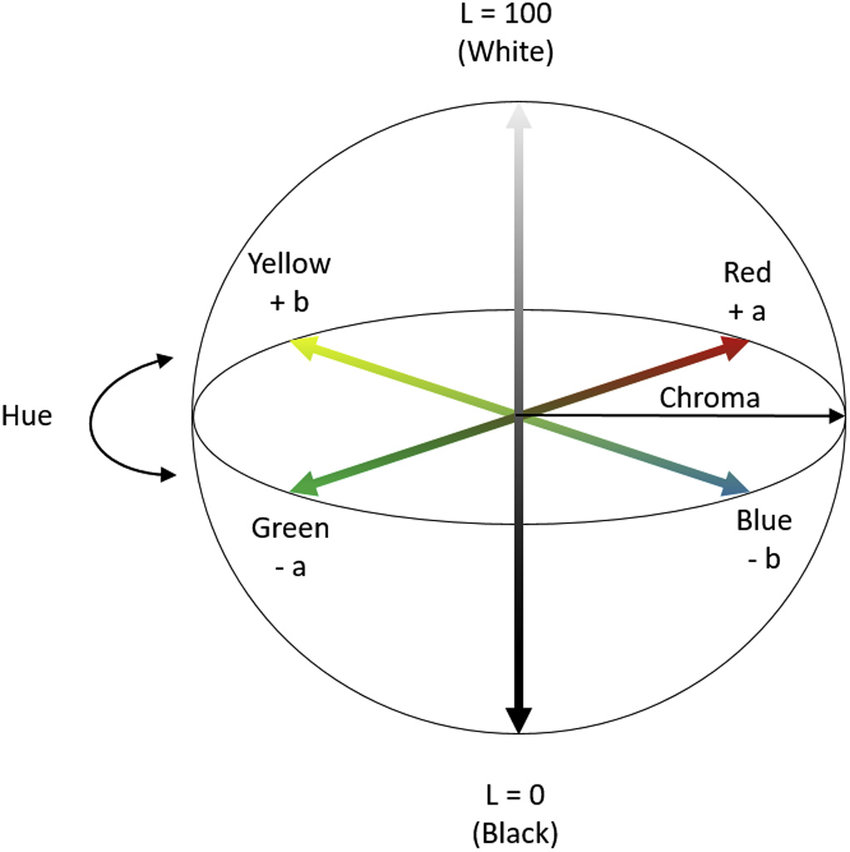
\includegraphics[width=0.4\textwidth]{2.png}
                        \caption{}
                        \label{model3}
                    \end{figure}

              \item Color histogram
                    \begin{itemize}
                        \item Try k-means clustering to find optimally different colors?
                    \end{itemize}
              \item Color space distance metrics
                    \begin{itemize}
                        \item Sum of absolute/squared distance
                        \item Euclidean distance
                    \end{itemize}
          \end{itemize}
    \item Build GAN with normal/color invariant discriminator
          \begin{itemize}
              \item Generate MNIST images
              \item Generate CIFAR-10 images
              \item Generate CelebA images (since they are higher dimensional with more discernible features)
              \item Test regular unsupervised learning models with generated images from both GANs
          \end{itemize}
\end{itemize}

\section{Technologies and Logistics}
We will implement the models in Python using the PyTorch library. We plan to do initial tests in the Google Colab environment but may have to move to Google Cloud Platform if the model testing becomes too demanding or for final large-scale tests. Regardless of platform, we plan to split the work such that we are all involved in the development and testing of the model. We have uncertainties about how the models may converge to local minima and not explore the greater color space. However, we expect to train a color invariant model that is able to handle unexpected colors significantly better than an equivalent model that does not use the novel color invariant modification we design.

\bibliographystyle{ieeetr}
\bibliography{bibliography}

\end{document}
